\documentclass{article}

\usepackage[utf8]{inputenc}		% obsluga jezyka polskiego
\usepackage[MeX]{polski}		%

\usepackage[top=1in, bottom=1.25in, left=1.25in, right=1.25in]{geometry}		%zmiana marginesów

\usepackage{graphicx}		%wyswietlanie obrazow
\usepackage{float}			%

\usepackage{rotating}		%obracanie obrazow
\usepackage{tikz}			%

\usepackage{multicol}		%tekst w kolumnach

\usepackage{listings}											%obsluga wyswietlania kodu
\usepackage{xcolor}												%
\lstset { %														%
	basicstyle=\ttfamily    									%
    language=C,													%
    backgroundcolor=\color{black!5}, % set backgroundcolor		%
    basicstyle=\footnotesize,% basic font setting				%
}																%
\usepackage{minted}												% obsluga wyswietlania kodu z kolorami

\renewcommand{\labelitemi}{--}			%zmiana wygladu znacznikow wypunktowania
\renewcommand{\labelitemii}{--}		%
%\usepackage[export]{adjustbox}

\begin{document}

\begin{titlepage} 
	\newcommand{\HRule}{\rule{\linewidth}{0.5mm}} 
	
	\center 
	
	%------------------------------------------------
	%	Headings
	%------------------------------------------------
	
	\textsc{\LARGE Politechnika Wrocławska}\\[1.5cm] % Main heading such as the name of your university/college
	
	\textsc{\Large Podstawy Techniki Mikroprocesorowej}\\[0.5cm] % Major heading such as course name
	
	\textsc{\large Dokumentacja techniczna projektu}\\[0.5cm] % Minor heading such as course title
	
	%------------------------------------------------
	%	Title
	%------------------------------------------------
	
	\HRule\\[0.4cm]
	
	{\huge\bfseries Nadajnik optycznddy sygnału Morse'a}\\[0.4cm] % Title of your document
	
	\HRule\\[1.5cm]
	
	%------------------------------------------------
	%	Author(s)
	%------------------------------------------------
	
	\begin{minipage}{0.5\textwidth}
		\begin{flushleft}
			\large
			\textit{Autor:}\\
			\textsc{Maciej Mielcarski} \\numer albumu: 235703\\~\\Wydział Elektroniki W-4\\Automatyka i Robotyka 
		\end{flushleft}
	\end{minipage}
	~
	\begin{minipage}{0.4\textwidth}
		\begin{flushright}
			\large
			\textit{Grupa zajęciowa:}\\
			\textsc{ŚR TP 13:15} 
		\end{flushright}
	\end{minipage}

\vfill\vfill\vfill % Position the date 3/4 down the remaining page
	
	{\large 15.04.2018 wersja projektu 1.0 } % Date, change the \today to a set date if you want to be precise 
	
\end{titlepage}



\pagenumbering{gobble}

  %\maketitle
  \newpage
\pagenumbering{arabic}  

\section{Wprowadzenie do projektu}
\subsection{Informacje ogólne}
Wykonany przeze mnie projekt obejmuje układ mikroprocesorowy, którego główna funkcjonalność dotyczy nadawania w formie optycznej sekwencji znaków standardu ASCII, wprowadzanych przez użytkownika za pośrednictwem interfejsu graficznego. Oprogramowanie mikrokontrolera zostało napisane w języku C.
\subsection{Wykaz elementów}
Układ, zmontowany na uniwersalnej płytce PCB zawiera następujące elementy wykonawcze:

\begin{itemize}
	\item	mikroprocesor 8-bitowy Atmega 32

	\item	wyświetlacz LCD rozdzielczości 8x2 znaki, zgodny ze standardem HD44780

	\item	mechaniczny enkoder obrotowy z wbudowanym przyciskiem

	\item	baterię 4 diod nadawczych LED, sterowanych tranzystorem NPN

	\item	2 przyciski monostabilne z układem redukcji drgań styków

	\item 	złącze IDC 10 SPI umożliwiające podłączenie programatora
\end{itemize}

\begin{figure}[h!]
	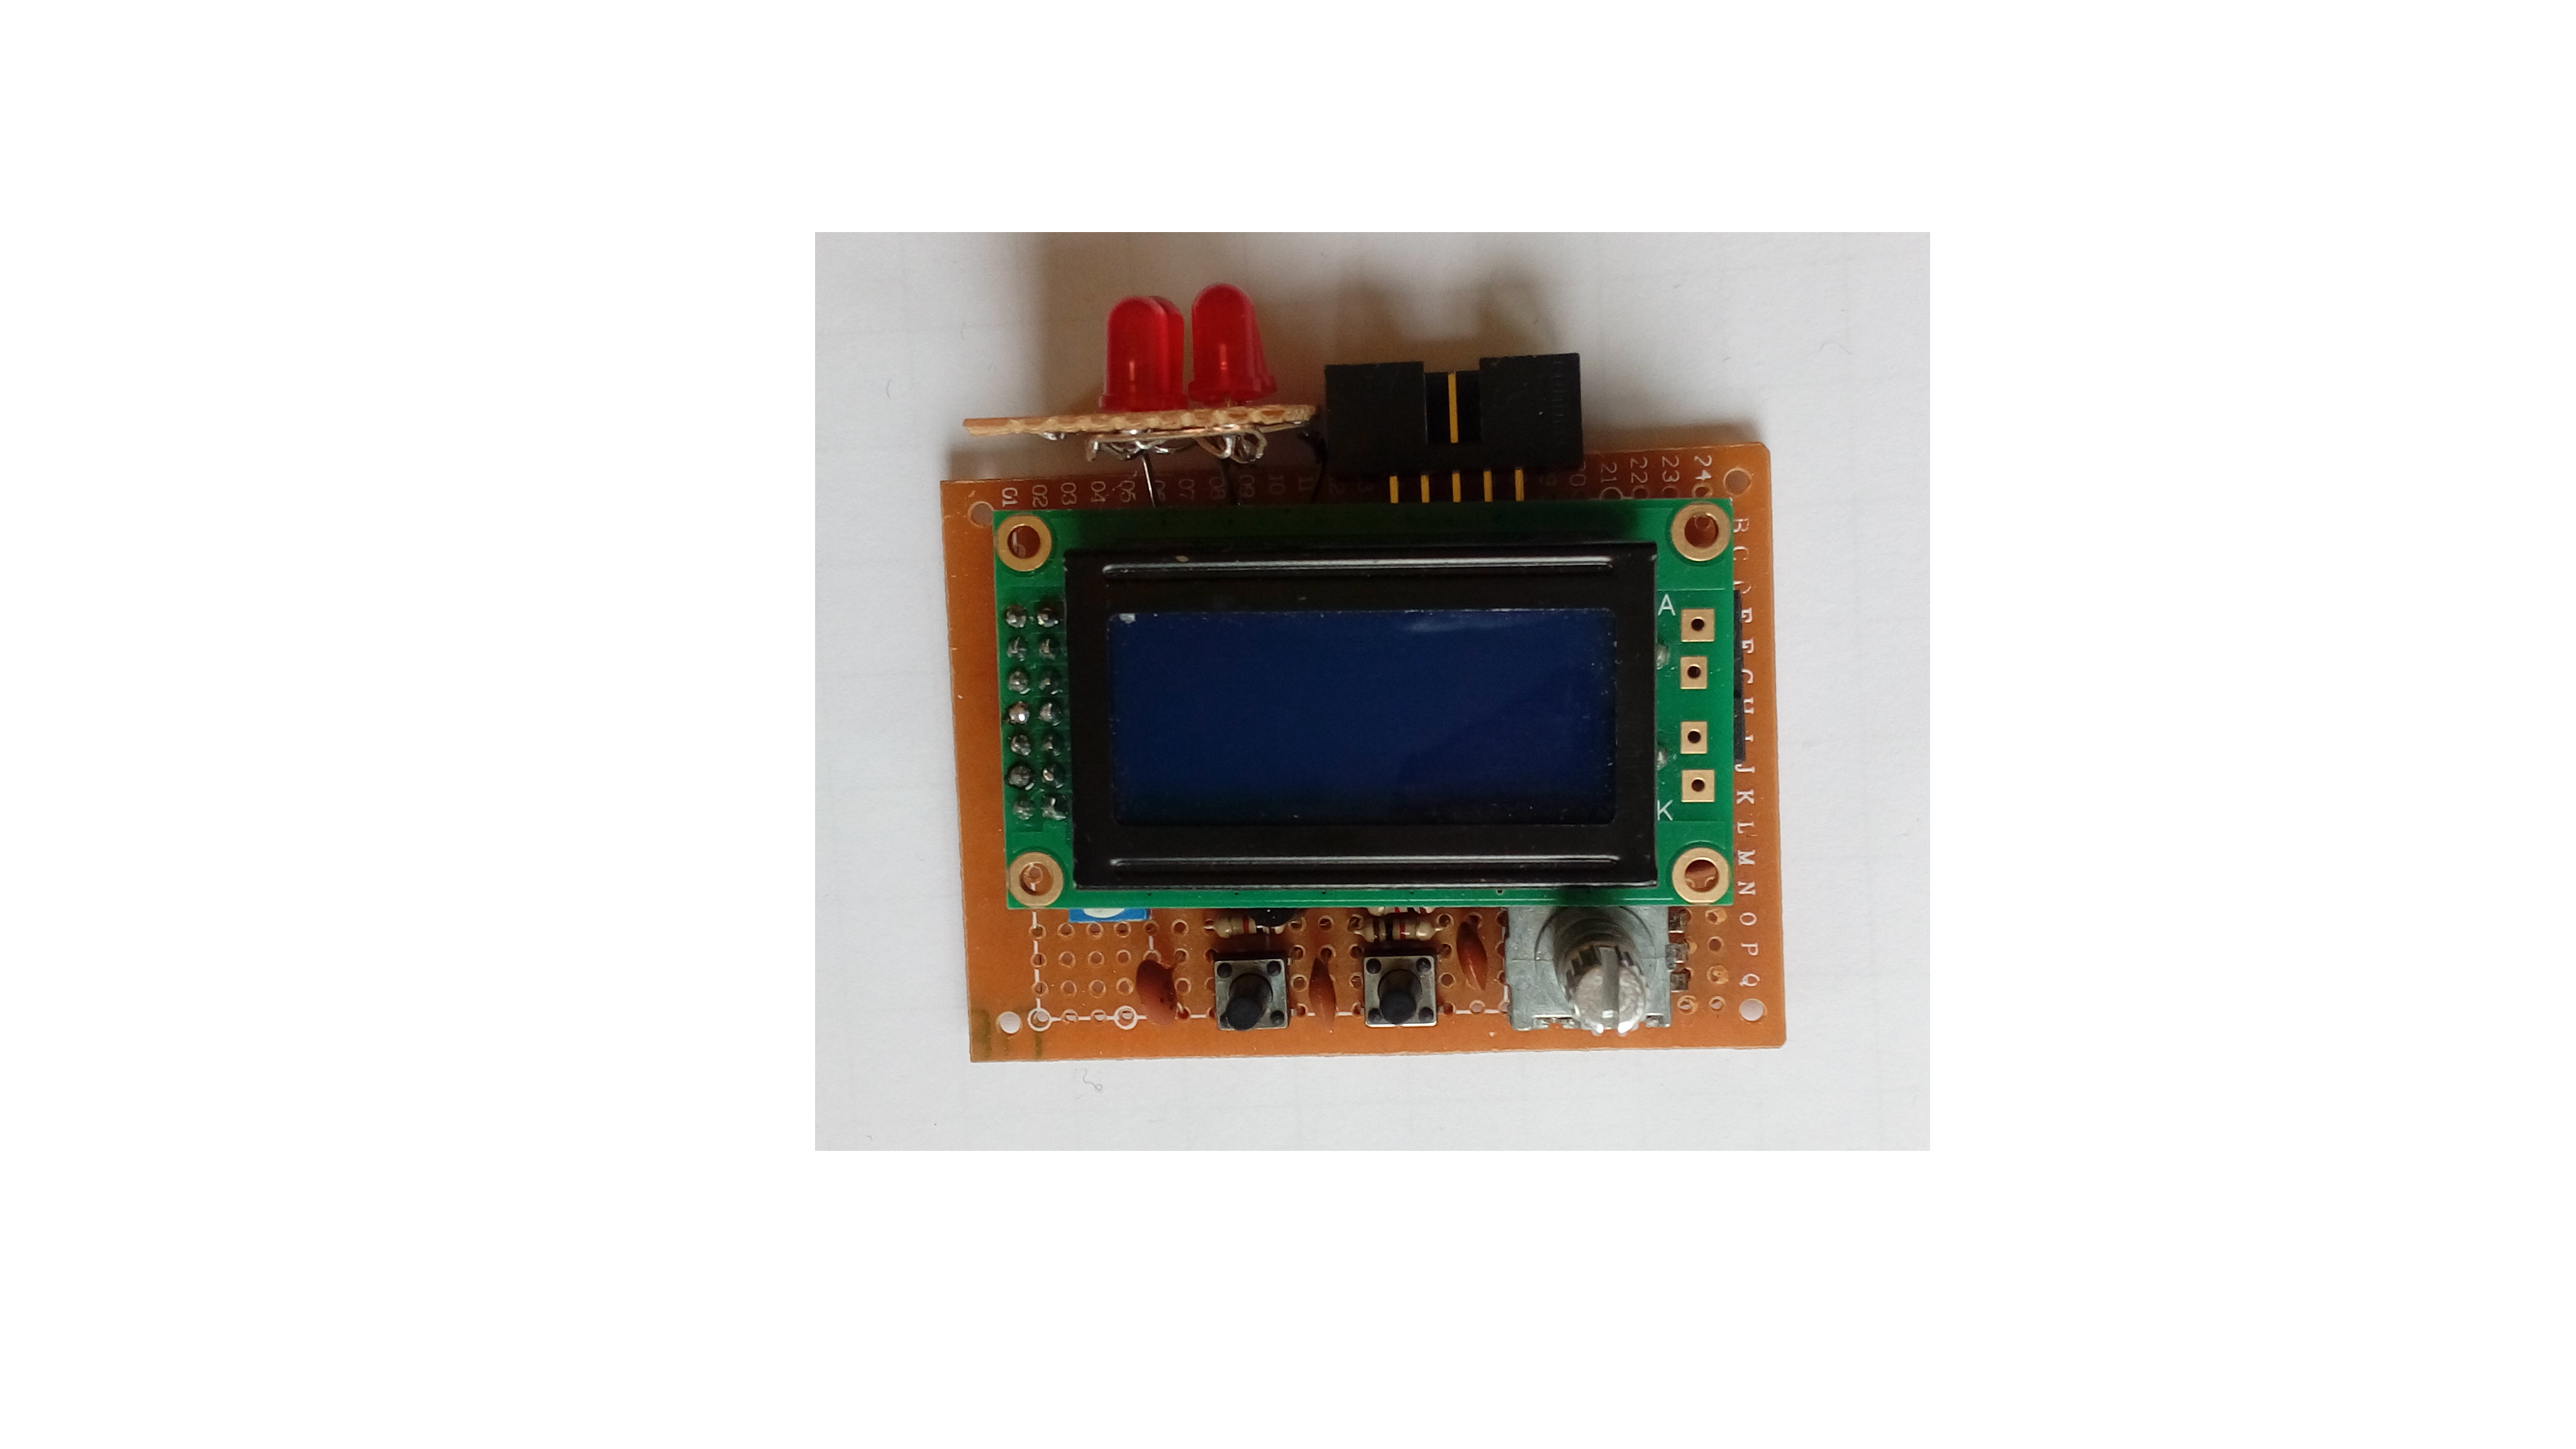
\includegraphics[width=\textwidth]{img/morse_main_view.png}
	\caption{Kompletne urządzenie nadajnika}
	\label{fig:zdjecie1}
\end{figure}

\newpage
\section{Konstrukcja układu elektronicznego}
\subsection{Schemat układu}
Schemat został przygotowany za pomocą programu KiCad 4.0.7. Układ składa się z mikrokontrolera wraz z filtracją zasilania, modułu wyświetlacza LCD z potencjometrem regulującym kontrast, złącza IDC 10 umożliwiającego aktualizację oprogramowania, modułu enkodera wraz z przyciskiem, czterech diod LED sterowanych tranzystorem NPN oraz dwóch przycisków monostabilnych. Pełen schemat przedstawiony na Rys. 4.

	
\subsection{Kluczowe moduły układu}
\subsubsection{Kompensacja drgania styków}
Znaczącym elementem układu jest filtr eliminujący tzw. "drgania styków" - zjawisko przełączania się styku w bardzo krótkim czasie pomiędzy stanem wysokim a niskim przy korzystaniu z przycisku. Jest to standardowy problem przy wykorzystaniu mechanicznych przełączników. Najbardziej popularnymi metodami kompensacji drgań są: metoda programowa oraz metoda sprzętowa. W pierwszym przypadku możemy zrezygnować z jakichkolwiek dodatkowych elementów wspomagających pracę przycisku i zastąpić je odpowiednimi funkcjami w programie, realizującmi opóźnienia wykonywania kodu po wykryciu pierwszej zmiany stanu przycisku. Jest to najtańsze rozwiązanie, lecz dodatkowo spowalnia i komplikuje działanie programu, a w przypadku układów czasu rzeczywistego, uniemożliwia nieprzerwaną pracę lub zajmuje przydatne do innych celów liczniki mikrokontrolera. Jeżeli jednak nie mamy problemu ze znalezieniem miejsca na płytce dla dodatkowego rezystora i kondensatora dla każdego przycisku, opcja sprzętowa jest odpowiednim dla nas rozwiązaniem. Kondensator podłączony równolegle do przycisku pełni rolę bufora, który naładowuje się w trakcie trwania drgań, uniemożliwiając pojawienie się w tym czasie stanu wysokiego na pinie mikrokontrolera. Rezystor podciągający napięcie zasilania możemy dodatkowo zastąpić odpowiednikiem programowym w celu minimalizacji elementów na płytce. 

\begin{figure}[h!]
	\center
	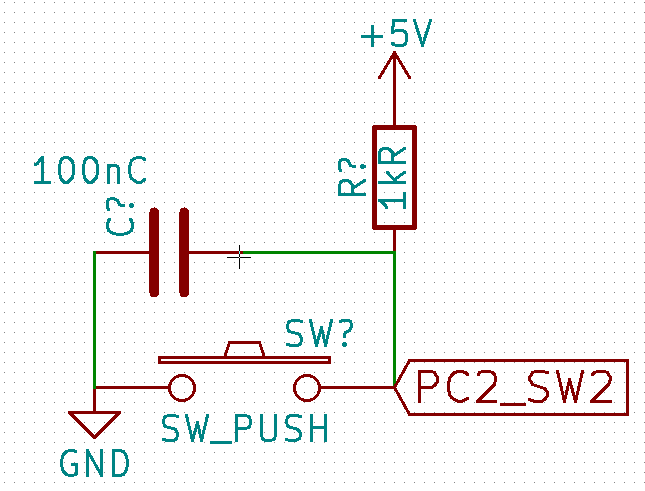
\includegraphics[scale=0.3]{img/drgania_stykow.png}
	\caption{Moduł przycisku monostabilnego z filtrem eliminującym drgania styków}
	\label{fig:zdjecie2}
\end{figure}

\newpage
\subsubsection{Sterowanie diodami nadawczymi}
W celu zapewnienia dobrej widoczności nadawanego sygnału zostały użyte 4 diody LED. Takie rozwiązanie nie pozwala jednak na sterowanie oświetleniem bezpośrednio poprzez mikrokontroler, przez niewystarczającą wydajność prądową jego wyprowadzeń. Dzięki zastosowaniu układu tranzystorowego, możemy w łatwy sposób sterować dużym prądem pobieranym przed diody poprzez mały prąd logiki mikrokontrolera. Napięcie zadawane na brankę tranzystora uaktywnia jego pracę, przepuszczając tym samym prąd pomiędzy zasilaniem a diodami. Niezbędne w takim układzie rezystory ograniczają prąd zarówno bramki tranzystora jak i ten płynący przez diody. 

\begin{figure}[h!]
	\center
	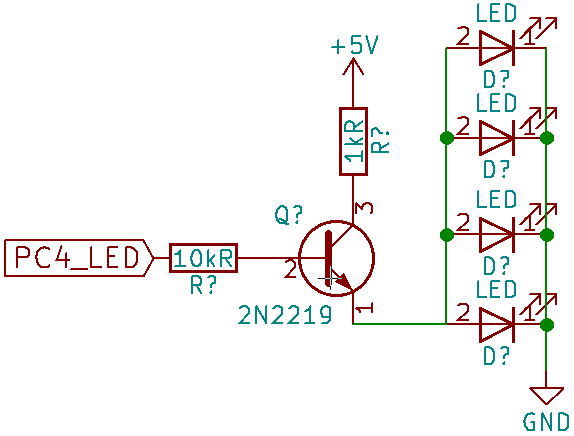
\includegraphics[scale=0.3]{img/sterowanie_diodami.png}
	\caption{Moduł sterowania diodami nadawczymi}
	\label{fig:zdjecie3}
\end{figure}

\section{Użytkowanie urządzenia}
Użytkownik obsługujący nadajnik Morse'a ma do dyspozycji szereg opcji związanych z nadawaniem i wyświetlaniem wiadomości. Interakcja z urządzeniem zachodzi poprzez obroty enkodera oraz 3 przyciski obsługujące zarówno długie jak i krótkie wciśnięcia.

\subsection{Menu główne}
Po uruchomieniu urządzenia użytkownikowi ukazuje się menu główne, obejmujące następujące pozycje:

\begin{itemize}
	\item	\textbf{nadaj}\newline
Opcja umozliwiająca wprowadzenie wiadomości za pośrednictwem obrotów enkodera oraz nadanie jej po wciśnięciu enkodera. Po skończeniu transmisji pojawia się komunikat pytający, czy powtórzyć nadawanie. Podczas transmisji wyświetlana jest sekwencja nadawanego kodu morse'a.

	\begin{itemize}
	\item uruchomienie opcji: wciśnięcie przycisku enkodera
	\item wybór znaku: obroty enkodera (zakres od a-z)
	\item zatwierdzenie znaku: wciśnięcie przycisku enkodera
	\item zatwierdzenie wiadomości: wciśnięcie przycisku enkodera przez co najmniej 2s
	\item powtórzenie nadawania: lewy lub prawy przycisk
	\end{itemize}

	\item	\textbf{wyswietl}\newline
Po wybraniu tej opcji, użytkownik ma okazję wyświetlić ostatnią nadaną przez niego wiadomość, zarówno w wersji znaków ASCII, jak i w kodzie morse'a. Za pomocą przycisków monostabilnych możliwe jest horyzontalne poruszanie się po wyświetlanej wiadomości. Wyjście z opcji przeglądania następuje po wciśnięciu przycisku enkodera.

	\begin{itemize}
	\item uruchomienie opcji: wciśnięcie przycisku enkodera
	\item przeglądanie wiadomości: lewy lub prawy przysik
	\item zakończenie opcji: wciśnięcie przycisku enkodera
	\end{itemize}

	\item	\textbf{rozszyf.}\newline
Jest to pozycja umożliwiająca wprowadzenie wiadomości w kodzie morse'a i przetworzenie jej na kod ASCII. Aktualnie nie jest dostępna, jednakże prace nad jej implementacją trwają.
	\item	\textbf{predk.}\newline
Za pomocą tej opcji możemy dostosować prędkość wyświetlanej przez nas wiadomości. Wartość ta wyrażana jest w słowach na minutę ( ang. wpm - words per minute), przy czym wartość 1 słowa na minutę oznacza prędkość wystarczającą do nadania słowa "PARIS" w ciągu jednej minuty (słowo "PARIS" zawira najbardziej standardowy przekrój liter w języku angielskim). Domyslnie, urządzenie nastawione jest na prędkość nadawania 10 wpm.

	\begin{itemize}
	\item uruchomienie opcji: wciśnięcie przycisku enkodera
	\item wybór prędkości: obroty enkodera
	\item zatwierdzenie prędkości: wciśnięcie przycisku enkodera
	\end{itemize}

\end{itemize}

\section{Kod programu}

\subsection{Główny pilk modułowy main.c}
\begin{multicols}{2}
%\lstset{tabsize=1}
%\begin{lstlisting}
\begin{minted}[tabsize=2,obeytabs]{c}
#include "morse.h"

int main(void){
	int menu = 0;		
	int btn = 0;		
	int menuEnc = 0;	
initializeSetup();
while(1)
{
	readEncoderCounter();
if(btn == 0)		
{
	if(encoderCount < 0) encoderCount = 0;	
	if(encoderCount > 3) encoderCount = 3;	
	menuEnc = encoderCount;
}
if(menu == 0)		
{
	LCD_Home();
	LCD_WriteText("Opcje:  ");
	LCD_GoTo(0,1);
	LCD_WriteText("Nadaj   ");
	menu=1;
}
else if(menu ==1)	
{
	switch (menuEnc)
	{
	case 0:				
		if(btn == 0)	
		{				
		LCD_GoTo(0,1);
		LCD_WriteText("nadaj   ");

			if(isButton())	
			{
				btn = 1;	
				LCD_Clear();
				encoderCount=0;
				delay_ms(800);
LCD_WriteCommand(
HD44780_DISPLAY_ONOFF 
| HD44780_DISPLAY_ON 
| HD44780_CURSOR_OFF 
| HD44780_CURSOR_NOBLINK);
			}
		}
			if(btn == 1)	
			{				
				if(dial())	
				{
				btn = 0;
				menu = 0;
				}
			}
	break;
	case 1:			
	if(btn == 0)
	{
	LCD_GoTo(0,1);
	LCD_WriteText("wyswietl");
		if(isButton())
		{
		btn = 2;			
		delay_ms(1000);
		messageDisplay();
		LCD_WriteCommand(
		HD44780_DISPLAY_ONOFF 
		| HD44780_DISPLAY_ON 
		| HD44780_CURSOR_OFF 
		| HD44780_CURSOR_NOBLINK);
		}
	}
	if(btn == 2)
	{
	LCD_moveMode();
		if(isButton())		
		{
		delay_ms(500);
		btn = 0;
		menu = 0;
		}
	}
	break;
		case 2:			
		if(btn == 0)
		{
		LCD_GoTo(0,1);
		LCD_WriteText("rozszyf.");
		
			if(isButton())
			{
			btn = 3;			
			LCD_Clear();
			delay_ms(600);
			encoderCount = 0;
			}
		}
		if(btn == 3)
		{	//messageDecrypt();
			/*if()
			{
				while(!(isButton()))
				{
					LCD_moveMode();
				}
			delay_ms(500);
			btn = 0;
			menu = 0;*/	
		}
	break;
		case 3:			
		if(btn == 0)
		{
		LCD_GoTo(0,1);
		LCD_WriteText("predkosc");

			if(isButton())
			{
			btn = 4;			
			LCD_Clear();
			delay_ms(600);
			encoderCount = 0;
			}
		}
		if(btn == 4)
		{
			if(setWpmSpeed())	
			{
			btn = 0;
			menu = 0;
			}
		}
	break;
		default:
	LCD_GoTo(0,1);
	LCD_WriteText("sw_err");
	menuEnc = 0;
	break;
	}}}}

\end{minted}
%\end{lstlisting}
\end{multicols}

\subsection{Plik modułowy morse.c}

\begin{multicols}{2}
%\lstset{tabsize=1}
%\begin{lstlisting}
\begin{minted}[tabsize=2,obeytabs]{c}
#include "morse.h"
extern int encoderCount = 0;		
extern uint8_t val=0;				
extern int asciiNum = 0;			
extern int wpmSpeed = 10;			
char lcdIntBuffer[4] = {};			
extern char userInput[30] = {};	
int morseInput[30] ={};				
int morseDecode[30] = {};			
char encodedMessage[30] = {};		
extern volatile uint16_t 
Timer1=0,
Timer2=0;	
int lcdPos = 0;						
extern int flag = 0;				
const uint8_t waitTime = 2;			
int btnFlag = 0;					
int encoderTmp = 0;					

const int morseTable[37][7] = {		
  {0, 1, 2},		//a
  {1, 0, 0, 0, 2},	//b
  {1, 0, 1, 0, 2},	//c
  {1, 0, 0, 2},		//d
  {0, 2},			//e
  {0, 0, 1, 0, 2},	//f
  {1, 0, 0, 2},		//g
  {0, 0, 0, 0, 2},	//h
  {0, 0, 2},		//i
  {0, 1, 1, 1, 2},	//j
  {1, 0, 1, 2},		//k
  {0, 1, 0, 0, 2},	//l
  {1, 1, 2},		//m
  {1, 0, 2},		//n
  {1, 1, 1, 2},		//o
  {0, 1, 1, 0, 2},	//p
  {1, 1, 0, 1, 2},	//q
  {0, 1, 0, 2},		//r
  {0, 0, 0, 2},		//s
  {1, 2},			//t
  {0, 0, 1, 2},		//u
  {0, 1, 1, 2},		//w
  {0, 0, 0, 1, 2},	//v
  {1, 0, 0, 1, 2},	//x
  {1, 0, 1, 2},		//y
  {1, 1, 0, 0, 2},	//z
  {0, 1, 1, 1, 1, 2},//1
  {0, 0, 1, 1, 1, 2},//2
  {0, 0, 0, 1, 1, 2},//3
  {0, 0, 0, 0, 1, 2},//4
  {0, 0, 0, 0, 0, 2},//5
  {1, 0, 0, 0, 0, 2},//6
  {1, 1, 0, 0, 0, 2},//7
  {1, 1, 1, 0, 0, 2},//8
  {1, 1, 1, 1, 0, 2},//9
  {1, 1, 1, 1, 1, 2}//0
  //0 - dot, 1 - dash, 2 - end
};

void initializeSetup (void)		
{
	 MCUCSR = (1<<JTD);			
	 //disabling JTAG
	 MCUCSR = (1<<JTD);			
	TCCR2 |= (1<<WGM21);						
	//work mode CTC
	TCCR2 |= (1<<CS22)|(1<<CS21)|(1<<CS20);		
	//prescaler = 1024
	OCR2  = 4;				
	//comparison interrupt every 10ms (100Hz)
	TIMSK = (1<<OCIE2);		
	//interrupt unlock CompareMatch

		DDRA &=~ (1 << ENC_A);		
		// encoder pins as input
		DDRA &=~ (1 << ENC_B);		
		PORTA |= (1 << ENC_B)		
		// with pull-up enabled
				|(1 << ENC_A);		

		DDRC |= (1<<LED);			
		//signal LED as output
		DDRA |= (0<<ENC_BTN);		
		//encoder button pin as input

		DDRC |= (0<<SW_1);	
		//switch 1 as input
		DDRC |= (0<<SW_2);	
		//switch 2 as input

	LCD_Initalize();		
	//LCD initializaion
	val = readEncoder();	
	//first encoder value reading
	sei();					
	//timers enabled
}

int dial(void)
{
	if(btnFlag == 0)
	{
		asciiNum = encoderCount+97;					
		if(asciiNum < 97) 	encoderCount = 25;		
		if(asciiNum > 122)	encoderCount = 0;		
		LCD_GoTo(lcdPos,0);
		LCD_WriteData(asciiNum);	
		LCD_GoTo(lcdPos,1);
		LCD_WriteData(94);			
	}

	/*if(!(PINC & 0x02) && !(PINC & 0x04))	
	{										
		LCD_Clear();
		return 1;
	}*/

	if (!(PINA & 0x08) && btnFlag == 0)		
	{
		Timer1 = (waitTime*1000)/10;		
		btnFlag = 1;						
	}
	else if((PINA & 0x08) && btnFlag == 1)	
	{
		userInput[lcdPos] = asciiNum;	 
		lcdPos++;						
		delay_ms(100);
		encoderCount = 0;		
		LCD_clearLine(1);
		btnFlag = 0;			
		Timer1 = 0;				
	}
else 
if(!(PINA & 0x08) && btnFlag==1&&!Timer1)	
	{
		LCD_Clear();
		userInput[lcdPos] = 'E';	
		for(int i=0;i<lcdPos;i++)	
		{
			LCD_GoTo(i,1);
			LCD_WriteData(userInput[i]);
		}
		//LCD_WriteData(lcdPos+48);
		btnFlag = 0;			
		delay_ms(1000);
		broadcast((2400/wpmSpeed),lcdPos);						
		delay_ms(700);
		btnFlag = 2;			
	}
	else if(btnFlag == 2)
	{
		LCD_Home();
		LCD_WriteText("powtorz?");
		LCD_GoTo(0,1);
		LCD_WriteText("T   N   ");
		if(!(PINC & 0x02))		//SW 1
		{
			LCD_Clear();
			delay_ms(500);
			broadcast((2400/wpmSpeed),lcdPos);
		}
		else if(!(PINC & 0x04))	//SW 2
		{
			lcdPos = 0;
			btnFlag = 0;
			return 1;
		}
	}
return 0;
}
void broadcast(int period,int length)
{
	int symbolSpace = period;
	int dashSpace = period*3;
	int charSpace = period*3;
	int wordSpace = period*7;
	int pos=0;
	for(int i=0;i<length;i++)
	{
		int j=0;
while(morseTable[userInput[i]-97][j]!=2)
		{
		LCD_GoTo(pos,0);
if(morseTable[userInput[i]-97][j] == 0)	
		{										//dot
			LCD_WriteData('1');
			morseInput[pos] = 1;
			blinkLed(period,symbolSpace);
		}
else if(morseTable[userInput[i]-97][j]==1)	
		{										//dash
			LCD_WriteData('0');
			morseInput[pos] = 0;
			blinkLed(dashSpace,symbolSpace);
		}
		j++;
		pos++;
		}
		delay_ms(charSpace - period);	
	}
	morseInput[pos] = 2;		
}

int setWpmSpeed()		
{
	wpmSpeed = encoderCount;
	itoa(wpmSpeed,lcdIntBuffer,10);				
	LCD_Home();
	LCD_WriteText("WPM:    ");
	LCD_GoTo(0,1);
	LCD_WriteText(lcdIntBuffer);
	if(isButton())
	{
		encoderCount = 0;
		delay_ms(600);
		return 1;
	}
	return 0;
}

void messageDisplay()	
{						
	LCD_clearLine(0);
	LCD_clearLine(1);
	if(userInput[0] < 97 
	|| userInput[0] > 122)
	{								
		LCD_Home();					
		LCD_WriteText("brak");
		LCD_GoTo(0,1);
		LCD_WriteText("danych");
		return;
	}
	int j = 0;
	while(morseInput[j] != 2)	
	{							
		LCD_GoTo(j,0);
		LCD_WriteData(morseInput[j]+48);
		j++;
	}
	int k = 0;
	while(userInput[k] != 'E')	
	{							
		LCD_GoTo(k,1);
		LCD_WriteData(userInput[k]);
		k++;
	}
}

void LCD_move(char dir)			
{
	if(dir =='L')				
	{
LCD_WriteCommand(
HD44780_DISPLAY_CURSOR_SHIFT
|HD44780_SHIFT_DISPLAY
|HD44780_SHIFT_RIGHT);
LCD_WriteCommand(
HD44780_DISPLAY_ONOFF 
| HD44780_DISPLAY_ON 
| HD44780_CURSOR_OFF 
| HD44780_CURSOR_NOBLINK);
		delay_ms(20);
	}
	else if(dir =='R')			
	{
LCD_WriteCommand(
HD44780_DISPLAY_CURSOR_SHIFT
|HD44780_SHIFT_DISPLAY
|HD44780_SHIFT_LEFT);
LCD_WriteCommand(
HD44780_DISPLAY_ONOFF 
| HD44780_DISPLAY_ON 
| HD44780_CURSOR_OFF 
| HD44780_CURSOR_NOBLINK);
		delay_ms(20);
	}
}

void LCD_moveMode()			
{
	if (!(PINC & 0x02))			
	{
		delay_ms(100);
		LCD_move('R');
	}

	if (!(PINC & 0x04))		
	{
		delay_ms(100);
		LCD_move('L');
	}
}

void blinkLed(int on, int off)	
{								
	PORTC |= (1<<LED);
	delay_ms(on);
	PORTC &= ~(1<<LED);
	delay_ms(off);
}

void delay_ms( int ms)			
{
	volatile long unsigned int i;
	for(i=0;i<ms;i++)
		_delay_ms(1);
}

void LCD_clearLine(int nr)		
{
		LCD_GoTo(0,nr);
		LCD_WriteText("        ");
}

int isButton()				
{
	if(!(PINA & 0x08))
		return 1;
	else	return 0;
}

uint8_t readEncoder(void)	
{
 uint8_t val=0;

  if(!bit_is_clear(PINA, ENC_B))
	val |= (1<<1);

  if(!bit_is_clear(PINA, ENC_A))
	val |= (1<<0);
  return val;
}

void readEncoderCounter ()		
{								
	uint8_t val_tmp = 0;						
	val_tmp = readEncoder();			

	if(val != val_tmp)
	{
		if((val==3 && val_tmp==1))
			{
			encoderCount ++;	
			}
		else if((val==2 && val_tmp==0))
			{
			encoderCount --;	
			}
		val = val_tmp;
		}
	delay_ms(1);
}

ISR(TIMER2_COMP_vect)	
{
	uint16_t n;
	n = Timer1;		
	if (n) Timer1 = --n;
	n = Timer2;		
	if (n) Timer2 = --n;
}
\end{minted}
%\end{lstlisting}
%\columnbreak
\end{multicols}

\section{Dalszy rozwój projektu}
Mimo sprawnej realizacji większości planowanych funkcji urządzenia, układ daleki jest od finalnej wersji. Po skonstruowaniu i przetestowaniu podstawowych czynności, układ jest gotowy do implementacji kolejnych etapów rozwoju, m.in.:
	\begin{itemize}
	\item dokończenie pracy nad funkcją rozszyfrowywania wiadomości
	
	\item przerojektowanie programu w celu zaimplementowania obiektów, takich jak przyciski, enkoder, opcje menu jako struktury (stworzenie szablonów do elementów wykonawczych, znacząco ułatwiło by to budowę kolejnych projektów)
	
	\item wprowadzenie możliwości nadawania paru wyrazów, trwałego zapisywania wiadomości oraz zapętlania przekazu	
	
	\item zaprojektowanie płytki drukowanej PCB wraz z obsługą zasilania baterią Li-Ion
	
	\item przebudowanie całości projektu do formy poręcznej latarki
	\end{itemize}

\begin{sidewaysfigure}[h!]
	\centering
	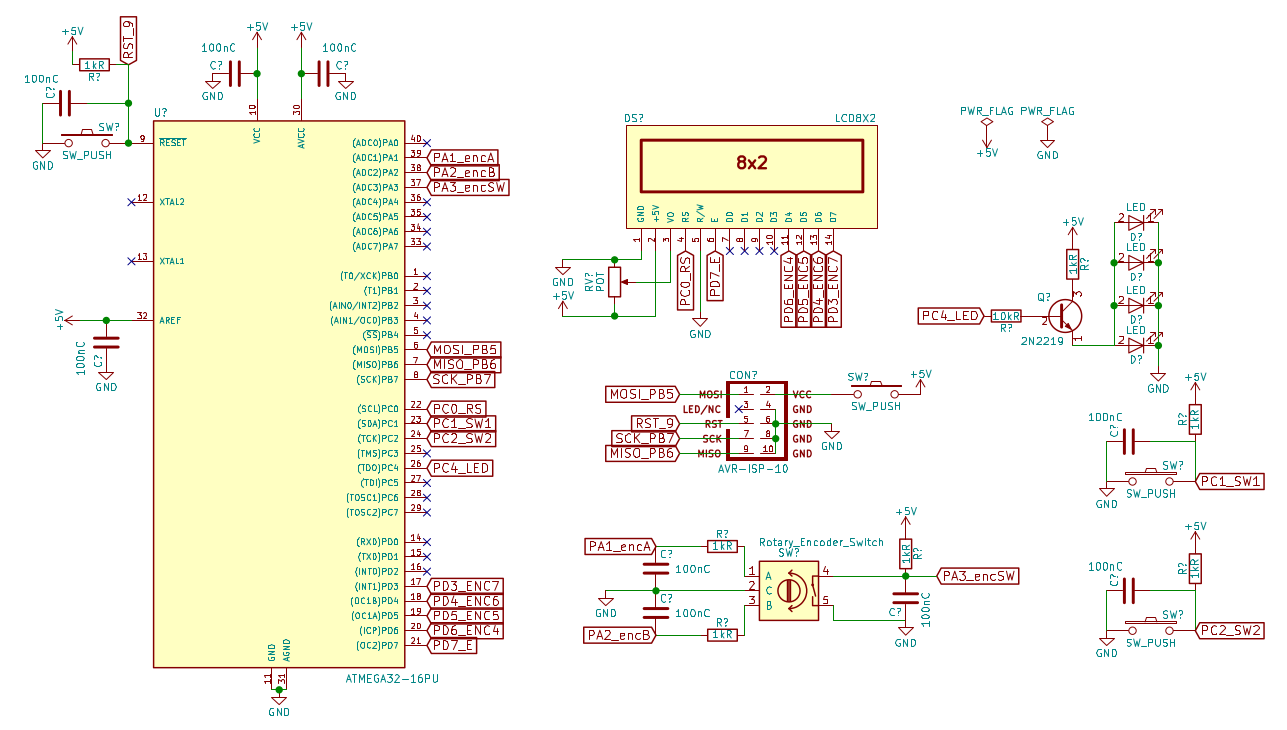
\includegraphics[width=\textwidth]{img/scheme.png}
	\caption{Schemat układu wykonany w programie KiCad}
	\label{fig:schemat1}
\end{sidewaysfigure}

\end{document}
